%! TEX root = **/010-main.tex
% vim: spell spelllang=en:

\subsection{Decision Trees}%
\label{sub:decision-trees}
\begin{figure}[H]
    \centering
    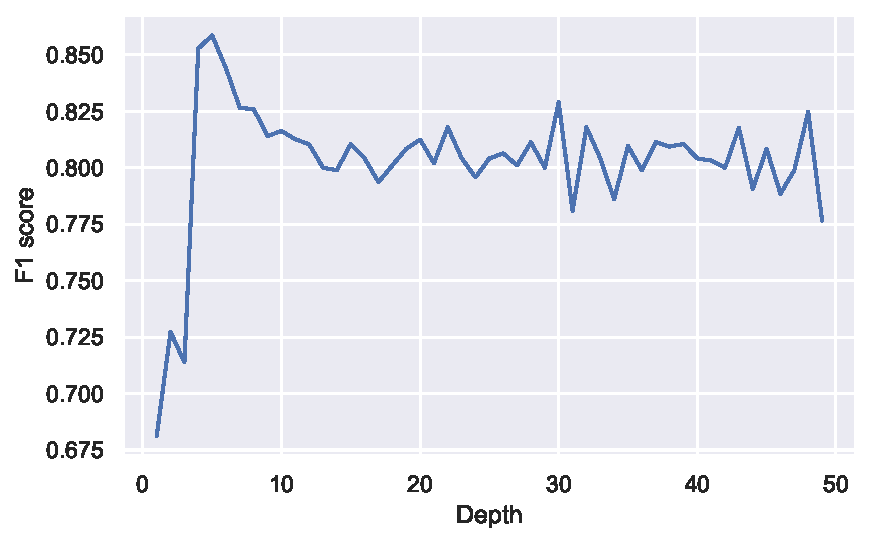
\includegraphics{decision_trees}
    \caption{decision trees accuracy depending on the depth.}%
    \label{fig:knn_pca_lda_nca}
\end{figure}

% Discussion of choice of parameters used. Try to interpret the obtained DT using some examples of the validation set. 
% Show some of the most relevant rules.  Discuss how + and – examples are mixed in leaves in order to
% estimate the reliability of the tree.